\section{Architecture}

\begin{figure}[t]
   \begin{center}
     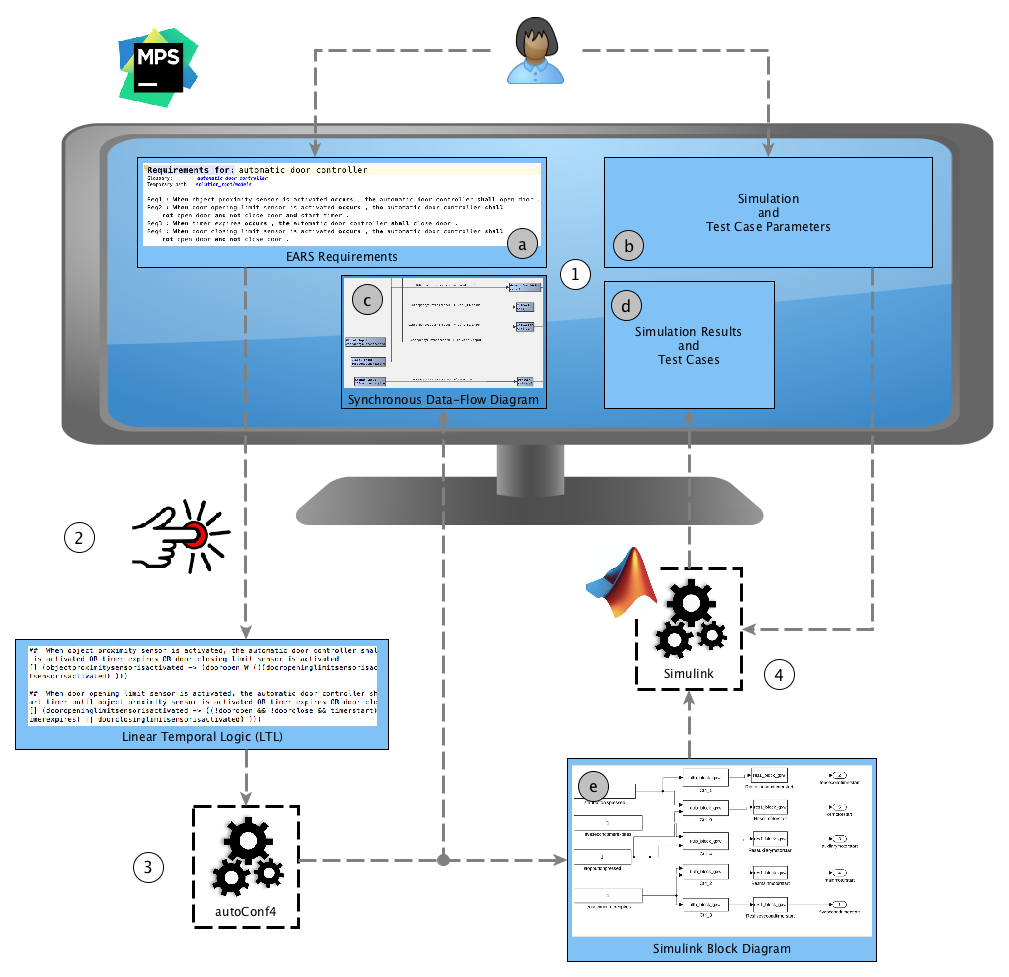
\includegraphics[width=1\textwidth]{images/toolchain.png}
     \caption{The \textsf{EARS-CTRL} Tool Chain\levi{finish pic}}
     \label{fig:ears_ctrl_toolchain}
   \end{center}
 \end{figure}
 
In figure~\ref{fig:ears_ctrl_toolchain} we depict the architecture of the
\textsf{EARS-CTRL} tool. In the following paragraphs we will provide the reader
a brief description of the main components of the tool's architecture, how those
components have been implemented as well as the artifacts they exchange. The
paragraphs are numbered such that each descriptions can be matched with the 
process-related components of the tool depicted in
figure~\ref{fig:ears_ctrl_toolchain}.
Additional letter-labels are used in figure~\ref{fig:ears_ctrl_toolchain} to
refer to data artifacts.
 
\paragraph{1. Editors and Control Panels\\\\} 

The requirements editor, the glossary editor, the simulation and test generation
control panel, the test generation control panel and the synchonous data-flow
diagram visualizer (respectively noted (\textsf{a}), (\textsf{b}), (\textsf{c})
and (\textsf{d}) in figure~\ref{fig:ears_ctrl_toolchain}) have all been built as 
domain-specific languages (DSLs) in the Meta Programming System (MPS) tool. MPS
is both a projectional editor and a domain-specific language workbench.
Domain-specific languages in MPS are composed of an abstract syntax (also known
as meta-model) and a concrete syntax. The concrete syntax allows displaying
and/or editing the information present in a model (as depicted for instance in
figures~\ref{fig:ears_reqs}, \ref{fig:ears_glossary} and
\ref{fig:ears_simulator}). Note that because MPS is a projectional editor, the
abstract syntax is directly edited which avoids an explicit or implicit
intermediate step where the concrete syntax is parsed.
A direct consequence of this is for example the fact that when a component's
name is updated an \textsf{EARS-CTRL} glossary, that update will immediately be
reflected in any requirements that refer to that component name. This automatic
update is an off-the-shelf feature of any editor defined using MPS and is an
easy way to guarantee that references between the several parts of an editor
always remain consistent.

\paragraph{2. From EARS to Lineal Temporal Logic\\\\}
\label{sec:ears_LTL} 

Let us consider the requirement \textsf{Req1} which is part of the
specification of the sliding doors controller in figure~\ref{fig:ears_reqs}:

\begin{center}
\textbf{When} \emph{object proximity sensor is activated} \textbf{then the} \emph{automatic door controller} \textbf{shall}
\emph{open door}.
\end{center}

 This requirement, taken in isolation, translates into the following LTL
 formula:
 
$$[] (objectproximitysensorisactivated \rightarrow dooropen)$$
which, if one takes into consideration the semantics of the $\rightarrow$
operator as ``implies'', is the expected logical meaning of \textsf{Req1}. All EARS
templates, when taken in isolation, can be directly translated into LTL and
propositional logic operators in such a straightforward manner.
If, however, one translates the whole set of requirements for the automatic
door in \ref{fig:ears_reqs} into LTL, the result for \textsf{Req1} will be as follows:

\begin{align*}
[] (object&proximitysensorisactivated \rightarrow\\
 &(dooropen\,W\,(dooropeninglimitsensorisactivated \lor timerexpires\\
 & \lor doorclosinglimitsensorisactivated )))
\end{align*}

This is due to the fact that the requirements specify behaviors that are
interwined during execution. For example, from \textsf{Req1}  in
figure~\ref{fig:ears_reqs} we know that if the \textsf{object proximity sensor}
is activated, the doors will open. We also know from \textsf{Req2} that, when
the \textsf{opening limit reached} sensor is activated, the doors will stop.
Without additional information, the \textsf{autoCode4} synthesis tool identifies
a contradition in these two requirements since, if the two sensors are activated
during the same execution, the doors will logically simultaneously open and
close. In order to avoid such contradictions it becomes necessary to establish a
temporal dependency between the behaviors specified by the requirements. In
order to achieve this our tool performs a static analysis of the requirements
in order to identify such dependencies and to add this information to the
generated LTL specification.
This additional contextual information in the generated LTL is clear from the
second translation above:
the door will only open, \emph{until} (the ``\textbf{W}'' operator) the door \textsf{opening limit
reached} sensor is activated, \emph{or} other events stated in related
requirements occur.
 
\paragraph{3. Synthesizing a Controller using \textsf{autoCode4}\\\\}
 
Controller synthesis is achieved via \textsf{autoCode4}'s Java API. The LTL
specification obtained as explained in section~\ref{sec:ears_LTL} is passed into
the synthesizer which returns a synchronous data-flow (SDF) diagram as an Java
object instance. The SDF diagram is then parsed and rebuilt as a visual model
which is an instance of the synchonous data-flow diagram visualizer DSL
(identified by label (\textsf{e}) in figure~\ref{fig:ears_reqs}). Such a visual
model provides the requirements engineer with a graphical and technical view of
the synthesized controller as a set of blocks and wires which can be used as a
debugging artifact.

\paragraph{4. Simulation and Test Generation using Simulink\\\\}

The SDF diagram obtained from the \textsf{autoCode4}
consists, for short, of a set of synchronized blocks that perform arithmetic,
logical or other functions on input signals and return the result on output signals. The controller's inputs and
outputs are also themselves represented as blocks. The fashion in which blocks
are synchronized is declared by connecting those blocks' inputs and outputs via
wires. In order to simulate \textsf{EARS-CTRL} specifications we have built a
translator from such data-flow diagrams onto Simulink models. Given that the SDF
formalism is very similar to the Simulink formalism, the structural translation
is essentially one-to-one. However, only a subset of all blocks present in
the SDF specifications that are produced by \textsf{autoCode4} is available
off-the-shelf in Simulink. As such, a number of Simulink blocks had to be built
by us to accommodate the semantics of SDF specifications. In
particular we had to build a number of stateful blocks to mimic in Simulink the
operation of some of SDF's blocks.

The Simulink model is generated by \textsf{EARS-CTRL} as a Mathlab simulink
script that builds the model programmatically (label \textsf{e} in
figure~\ref{fig:ears_reqs}). Communication with simulink from the \textsf{EARS-CTRL} IDE for
simulation and test case generation is also programatically achieved through the
use of the \textsf{mathlabcontrol}\cite{mathlabcontrol} Java API.
